\documentclass[11pt,a5paper]{book}
\usepackage{alltt}
\usepackage{ascmac}
\usepackage[dvipdfmx]{graphicx}
\usepackage{eclbkbox}

\title{トレーニング・フォア・データライブラリアン}
\author{天野晃}

\begin{document}
\maketitle
\tableofcontents

\part{導入}
\chapter{対象読者}
本書が対象とする読者は、現職の図書館員、または、相当の業務(研究支援等)を行う職員である。
広くは研究所や大学の情報及び図書に関わる部門において研究データを取り扱う業務に従事するものである。
前提としている知識・技術として、コマンドラインシェルを扱え、簡単なプログラム(スクリプト)が組める。
例えば、UNIXユーザーならbash、WindowsユーザーならPowershellを利用し、複数のプログラムを呼び出し、パイプライン化を行うようなことがすでに身についていることを前提としている。
また、データベースの知識があることが望ましい(利用経験はなくて良い)。
本書は「一冊で終わる」本ではない。エッセンスのみを凝縮させたような、いわば、学習の起点となるような本を目指した。その目的から言えば深い理解を目指しているわけでもなく、研究者とデータについて語り合える最低限の計算機とデータの知識・技術を提示しているにすぎない。しかしながら、あるいはそれだけに、バランスの良い、一種の入門書としての存在となることを目指した。


\chapter{図書館員を取り巻く状況}
\section{データサイエンティストとデータライブラリアン}
データライブラリアンと同様にデータに深く関わる職としてデータサイエンティストと言われるものがある。
近年、研究におけるデータ管理・公開の重要性が強く認識されるようになり、これらの職種に対して注目と期待が集まっているが、
一つの差別化の考えとしては、
データサイエンティストはあくまでも研究者であり、研究対象がたまたまデータであるに過ぎないと考えることができる。
この意味において、他の研究者と同様、常にライブラリアンの助けを必要としている。


\section{想定するデータライブラリアンの仕事}
データライブラリアンは、研究者が研究活動に専念できるように様々なサポートを行なうべき存在である。
雑誌契約やレファレンス、図書受け入れ作業などと同格な業務として、データ利用契約、データ検索、登録データのチェック、公開データの構造化、これらに関わるシステムの設計、ツールの作成などといった作業を行うことになるであろうことが予想され、業務の目的としては何ら今までのライブラリアンの仕事と変わらない。

ただ、技術面に注目すれば、このような作業を行うには、各分野におけるデータの性質に関する知識があることに加え、データチェックのための技能、データを構造化するための知識やデータ構造の解析技術などが身についている必要がある。
また、このような様々な形態のデータを処理するにあたり、毎回対応するスクリプティングやプログラミングを行うことは非効率的であり、これらのデータを効率的に扱うことができる高機能なツールは必須である。
しかしながら、逆説的ではあるが、高機能なツールでは処理が重すぎて利用が困難な場合もある。
つまり上記の業務を効率的に行うには、いずれの場合にも対応できるように、それぞれのツールに対する知識が必要となる。
本書によって、これらのツールや機能を使いこなすための、データに対する知識とデータ処理の基本的な考え方が身につくことを期待している。


\part{基礎技術編}
\chapter{計算機とデータの知識}
\section{データとは}
データとは、計算機が扱うことのできる情報の形式と考えることができる。
この意味では、データを理解するためには計算機の構造をある程度理解する必要があることを述べておく。
このことは「データ処理とは」の章でもう少し詳しく解説するが、本書では端的には「電子計算機が扱うことのできるバイト列またはビット列」を指す。
\begin{breakbox}
$\Rightarrow$ 電子計算機以外にどのようなタイプの計算機があるか調べてみよう。
\end{breakbox}

\subsection{データ型}
一般的にデータ型とはデジタル電子計算機が扱うデータフォーマットのことと考えてよい。データ型には幾つかの抽象化レベルがあるが、最下層としては単なるビット列をどのように解釈するかである。すなわち、例えば以下のようなものである。
\begin{itemize}
\item 整数型
\item 小数(浮動小数点数)型
\item 文字型
\end{itemize}
\begin{breakbox}
$\Rightarrow$ 上記以外にどのようなデータ型があるか調べてみよう。
\end{breakbox}

\subsection{文字と文字列}
ここで、文字と数字、文字列について述べておこう。
文字は文字コードによって解釈されるが、文字コードはさらにエンコードされている。
UTF8とは、ユニコードをエンコードする一つの方法である。数字とは、数を表すための文字であり、数値とは異なる。
数値とは前述したように、整数や小数という概念そのもの、あるいは計算機上で数値として取り扱うビット列のことである。
文字列とは文字コードまたは文字エンコードの並らびである。
数値は、数字列によって表現されることが一般的である。
直接バイナリ記述される場合もある。
\begin{breakbox}
$\Rightarrow$ このことをCの\shortstack[l]{sscanf()}などで確認しよう。

$\Rightarrow$ リトルエンディアンとは何か調べてみよう。
\end{breakbox}

\subsection{集合、リスト、ツリー、グラフ}
\begin{figure}
\begin{center}

\begin{tabular}{c}
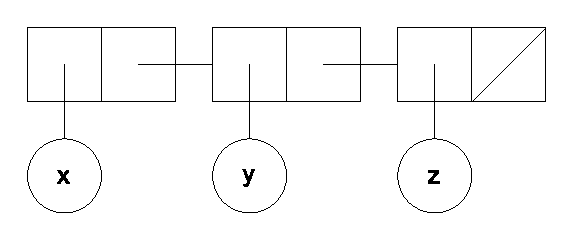
\includegraphics[width=8cm]{list_xyz.eps} \\
�ꥹ��(x,y,z)��ɽ�����ꥹ�ȹ�¤ \\
\\
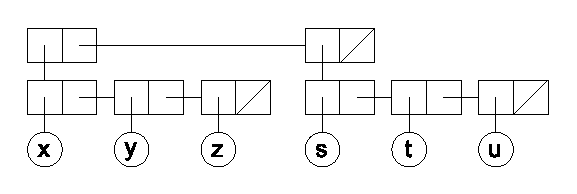
\includegraphics[width=8cm]{list_xyz-stu.eps} \\
�ꥹ��((x,y,z),(s,t,u))��ɽ�����ꥹ�ȹ�¤(����) \\
\end{tabular}

\caption{\label{zu-cell} [�ꥹ�ȹ�¤]}
\end{center}
\end{figure}

\begin{figure}[h]
\begin{center}

\begin{tabular}{c}
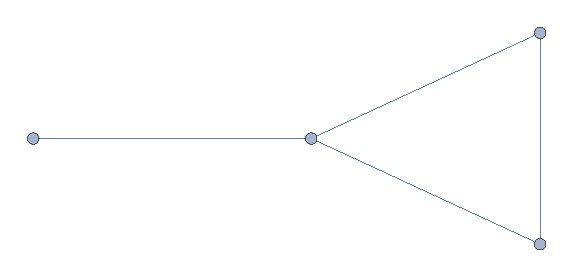
\includegraphics[width=8cm]{zu-gr.eps} \\
����դΥ���ե�����ɽ�� \\
\\
%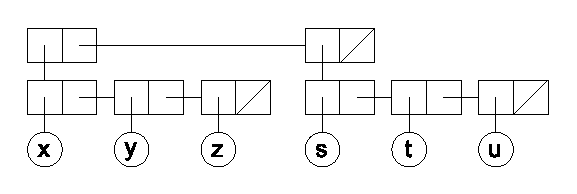
\includegraphics[width=8cm]{list_xyz-stu.eps} \\
\begin{math}
\left(
\begin{array}{cccc}
 0 & 1 & 1 & 1 \\
 1 & 0 & 0 & 0 \\
 1 & 0 & 0 & 1 \\
 1 & 0 & 1 & 0 \\
\end{array}
\right)
\end{math} \\
����դ����ܹ���ɽ�� \\
\end{tabular}

\caption{\label{zu-graph} [����չ�¤]}
\end{center}
\end{figure}

一般的にデータを取り扱う際にはデータ単体(datum)の単位では扱わず、データ集合として扱う。
ここで言う集合は一般的な集合ではなく、一種の配列、つまり、要素の並び順や重複に意味があるものである。
リストとは、要素を並べただけのものから、より高位の階層構造などを表すために用いられる表現である。
最も代表的な構造はCons Cellであり、文字列による表現ではカッコ()によって階層を表し、内部実装としてはポインタによるセルの連結である[Figure:\ref{zu-cell}]。
近年よく用いられるJSON形式は一種のリスト表現である。
ツリーは基本的にはリストと同じで、分岐のあるリストを特にツリーと称する。
この場合も内部実装はCons Cellで現すことができる。
グラフはより高位の構造であり、抽象レベルの表現、内部実装ともに複雑になるが、これらを表現する幾つかの方法がある。
その一つは隣接行列を利用することである[Figure:\ref{zu-graph}]。

グラフよりもさらに高次な構造も当然ある。
グラフの均質化やラベル付与は、より複雑なネットワーク構造を表す\cite{FujiwaraYuzuru}。
いずれの構造を表わすにおいても、前述のリスト構造がデータ構造における基本と考えてよい。

\begin{breakbox}
$\Rightarrow$ 配列とポインタ参照 \\
プログラミング言語ではよくポインタが使用されるが、Javaのような近代的な言語はその効果が隠蔽されており、解り難い。
C言語においてすらポインタ参照と配列参照はカッコ[]と引数で表現され、違いがない。
しかし、次のようなコードでその違いを確認できる。
\begin{center}
==========Start of code==========
\end{center}
\scriptsize
\begin{verbatim}
/* データサイズをprintする */
#include <stdio.h>
#include <stdlib.h>

int main(){
        printf("int             \t:%ld:\tbyte\n",sizeof(int));
          int a[2][2];
        printf("int 2D:2x2      \t:%ld:\tbyte\n",sizeof(a));
        printf("pointer int*    \t:%ld:\tbyte\n",sizeof(int*));
        return(0);
}
\end{verbatim}
\normalsize
\begin{center}
==========End of code==========
\end{center}
出力は以下となる。
\begin{center}
==========Start of print==========
\end{center}
\scriptsize
\begin{verbatim}
int             	:4:	byte
int 2D:2x2      	:16:	byte
pointer int*    	:8:	byte
\end{verbatim}
\normalsize
\begin{center}
==========End of print==========
\end{center}
\end{breakbox}

\subsection{メタデータ}
蛇足ながら、メタデータについて述べておく。
メタデータはデータを説明するためのデータであり、何がメタデータであるかは、個々のシステム、個人により定義されるが、明確に定義されない場合もある。
データが形式的になるほど、何がメタデータで何がデータなのかという区別は不要になっる。
すなわち、データ構造が完全に形式的に定義され、その解釈も一意に決まる場面では、メタデータという概念は不要である。


\section{データ処理とは}
データ処理とは、計算機が扱うことのできる情報の変換である。
より詳細には、処理対象と処理命令の定義が記述された表現を、その表現以外の知識(ルール)を用い、表現が変化しなくなるまで評価を続けることであり、すなわち、端的には「表現評価系を用いた表現の変換」と言える。
この解釈では「処理命令」(=プログラム)と「処理対象」(=データ)は分離が曖昧であり、計算機科学としてはどちらも「処理対象」とすることがふさわしい。
このことは、より抽象的かつ厳密に万能チューリングマシンとして定義可能である。
\subsection{チューリングマシン}
チューリングマシンとは、アラン・チューリングによる仮想機械の仕組みであり、現実の計算機はこれを物理的に実装したものであり、次の要素から成る。
\begin{itemize}
\item 状態(有限)を記憶するメモリ
\item 記号(有限)列(無限)を記録するテープ
\item メモリとテープを読み書きするデバイス
\end{itemize}
なお、チューリングマシンの論理的表現の要素は以下となる。
\begin{itemize}
\item $M$: 状態を表す有限集合
\item $T$: 記号集合
\item $\delta$: $\delta(m,t) = (m', t', h)$: 遷移関数、ただし、$m,m' \ni M$、$t,t' \ni T$、$h$: テープの移動方向
\end{itemize}
つまり、マシンは現在の状態($m$、$t$)を読み、遷移関数の定義に従い次の状態($m'$、$t'$)を作り、どちらかに移動し、これを繰り返す。
ただし、以上は最も簡単な構造であり、より複雑な多次元テープと複数デバイスのモデルも構築することができる。
実際の計算機は万能チューリングマシン、つまり、他のチューリングマシンをエミュレート可能なチューリングマシンとして設計実装されており、基本的には上記の考えを拡張したものである。
\begin{breakbox}
$\Rightarrow$ WolframAlpahを利用してチューリングマシンの動きを確かめよう。
\end{breakbox}

\subsection{セルオートマトン}
一方、局所規則のみで自己組織的に駆動する構造がセルオートマトンである。一部の規則群がチューリング完全である。つまり、適切な規則を定義することによりチューリングマシンとして機能する。
\begin{figure}[h]
\begin{center}
\begin{tabular}{c}
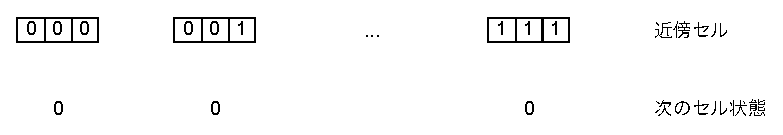
\includegraphics[width=8cm]{zu-ca.eps} \\
���륪���ȥޥȥ�(1����2��˵2����)���Ѳ���§�ΰ��\\
\end{tabular}
\caption{\label{zu-ca} [���륪���ȥޥȥ�]}
\end{center}
\end{figure}

セルオートマトンは、n次元のセル構造とセルの取り得る状態とセル状態の変化規則からなる。
例えば、「1次元3近傍2状態」とは、一次元に並ぶ有限または無限のセルと、変化規則が適応される3つの連続したセル(うち真ん中の一つは自分自身$=$状態変化の対象)のパターンからなる。
このとき、8通り($=2^3$)の状態からの遷移を規定しなければならず、すべての変化規則は256($=2^8$)通りとなる[Figure:\ref{zu-ca}]。
\begin{breakbox}$\Rightarrow$
2次元9近傍2状態の変化規則が何通りか考えよう。
\end{breakbox}

\subsection{プログラミングとは}
プログラミングとは、計算機に対しての処理命令をまとめたものであり、プログラミング言語はそれを行うための仕組みの一つである。
広義には、人間または計算機が、計算機に指示をするための様々なレベルの様々な仕組みであり、簡単なバッチ処理スクリプトや、たった一つの機械語命令もこれに含まれる。
しかし、より狭義には次のような特徴を持つプログラミング言語を用いて行うものが、プログラミングであると考えるのが妥当であろう。
\begin{itemize}
  \item 抽象化
  \item 繰り返しまたは再帰
  \item 条件分岐
\end{itemize}
抽象化とは、変数を利用可能であることである。ポインタの利用も抽象化の一種である。
繰り返しと再帰は、本質的に同等であり、相互に書き換えが可能であるとされる。
条件分岐は、最も直感的に必要であると考え得る機能のはずである。
\begin{breakbox}$\Rightarrow$
マークアップ言語(HTMLやYML)がプログラミング言語であり得るか、考えてみよう。
\end{breakbox}



\section{データ処理の基本技術}
\subsection{文字列処理}
文字列処理の中心はパターンマッチおよび文字(列)書き換えの技術である。
パターンとは、特定の文字列または文字列集合を表すもので、多くの場合、このパターンそのものが文字列として表現される。
とくに、文字列集合を一つの文字列で表す方式を正規表現または正則表現と言う。
現在では、正規表現はライブラリ(エンジン)として纏められ、共通ライブラリが複数のユーティリティーで利用されている。
Perl互換正規表現ライブラリ(PCRE)と鬼車(Oniguruma)は代表的な正規表現ライブラリである。

一方で、バッカス・ナウア記法(BNF)は、文法定義のためのメタ言語である。すなわち与えられた文字列がその言語において受け入れられるかを決定するための表現である。

さらに、マークアップ言語もマークアップ言語に対する定義を表すスキーマ言語も、メタ言語として捉えることが可能である。

上記のいずれの表現も、文字列パターン定義および文字列処理定義に利用可能である。
\begin{breakbox}$\Rightarrow$
正規表現、BNF(文法定義記法)、マークアップ言語、に対するユーティリティーに何があるか調べてみよう。
\end{breakbox}

\subsection{数値処理}
数値処理は、有限精度の値の計算結果を、有限精度の値として出力する。
数値の精度はハードウエアによって決まるが、有限精度の値を配列させることにより任意精度の計算も可能となる。
この際の精度とは、純粋に表現可能なビット数である。
さらに、表現されているビット列が、どの程度確からしいかを表す言葉として、確度というものがある。
すなわち、ある数値が表現されいている時、この裏には精度や確度といった情報が隠れていることになる。

基本的に、実際の数値計算においては、計算を重ねるごとに確からしさが減少する。

\subsection{数式処理}
数式処理とは、数値処理を含むより広義な、Symbolic Computation System や、Computer Algebra System 等の概念を含むもので、実装としては、Mathematica、Mapleといった商用アプリケーション、Maximaのようなオープンソースが存在する。

Symbolic Computation System は、記号(symbol)を、何らかの変数記号として、数値の代入を行うことなく可能な処理を行う。例えば、代数処理として$a - a$の表現を$0$として評価する。この例では記号に対して代数処理が行われており、前述のアプリケーションに代表されるシステムにおいても、記号的な代数システムが用いられている。

\begin{breakbox}$\Rightarrow$
テスト用。
\end{breakbox}


\chapter{統計または解析の技術}

\chapter{表示・表現の技術}

\part{実践編}
\chapter{サービス構築}
\section{データベース}
\section{HTTPサーバー}

\chapter{データ解析}

\bibliographystyle{plain}
\bibliography{My_Collection.euc}


\end{document}

